\section{Implementation}

This chapter will discuss how our datasets, embeddings and various models were created using the decisions made in Chapter \ref{sec:Design}.

\subsection{Drug-Target Interactions Dataset}

To create our DTIs dataset we started by downloading all the predicted human proteins from the AlphaFold protein structure database \citep{Jumper2021, Varadi2022} and retrieving all the protein accession numbers and sequences. Then using these protein accession numbers \citet{PubChemAPI} calls were made to retrieve the DTIs associated with each protein.

Some proteins had thousands of DTIs available and we felt including every single one would be not only difficult but also counterproductive. Therefore, we decided to place a limit on the number of DTIs retrieved for each protein. This number was arbitrarily set to 100 and if a particular protein's DTIs exceeded that then we would randomly select 100 of them.

Once we had our DTIs it was time to retrieve the descriptors associated with each drug and protein sequence. For each drug we again made use of \citet{PubChemAPI} calls to retrieve every single chemical descriptor stored by PubChem \citep{PubChem}. 

For each protein we used the Protr \citep{ProtR_Paper} library as mentioned in Subsection \ref{subsec:Protein_Sequence_Descriptors} to calculate a large selection of protein sequence descriptors from a variety of descriptors families and UniProt \citep{UniProt_Paper} to extract each protein's sequence embedding. We decided to use a variety of protein sequence descriptor families instead of focusing on a single one because, as we have already discussed in Subsection \ref{subsubsec:Important_Protein_Sequence_Descriptors}, a combination of them can enhance our models' predictive performance.

Once we had everything we needed we performed data cleaning, removing any protein without any DTIs discovered and any dataset entry with missing descriptors, drug or protein related. This process decreased the size of our dataset from 190,028 DTIs to 163,080, with 112,597 classified as having an active relationship and the remaining 50,483 classified as having an inactive one. 

As for the entries having binding affinity available, 72,908 had $IC_{50}$ available, but with just 14 of these being classified as inactive. This was clearly not diverse enough and therefore we moved on to the second most common binding affinity which was $K_d$, with 20,372 entries, 15,007 classified as having an active relationship and 5,365 classified as having an inactive one.

\subsubsection{Feature Selection}
\label{subsubsec:Feature_Selection}

To improve our models' predictive performance, training times but to also discover the drug and protein sequence descriptors holding the most predictive power we decided to use the recursive feature elimination with cross-validation function (RFECV) offered by Scikit-Learn with a random forest classifier or regressor depending on the dataset we would be using and 5-fold cross-validation.

Before running RFECV we decided to reduce the number of tripeptide protein sequence descriptors using principal component analysis (PCA), a dimensionality reduction method, to reduce their size to a number holding 95\% of their variance. As a result, PCA managed to reduce the tripeptide descriptors from 8000 to 2616.

RFECV managed to reduce the features for the classification dataset from 6,474 to 388 and for the regression dataset from 6,474 to 693. 

\subsection{Holdout Test Sets}

As mentioned in Subsection \ref{subsubsec:Model_Evaluation} we decided to use holdout test sets to evaluate our models with previously unseen data. To achieve this we used the train test split function from Scikit-Learn.

Given the nature of our dataset, many proteins can be associated with many drugs, so we could not do the traditional 80/20 split. What we chose to do instead was to take a small subset of our dataset as our test set and remove any proteins and drugs associated with it from the training set. This naturally led to some entries from the dataset not being utilised at all, but we were still left with a substantial amount of training and test data.

For our classification models the training set was 99,705 DTIs and the test set was 816 DTIs and for our regression models the training set was 10,956 DTIs and the test set was 102 DTIs. The same holdout test set will be used for both baseline and enhanced models in order to compare them properly. However, we expect to lose some entries when testing the enhanced models due to not being able to create embeddings for every single protein present in the dataset.

\subsection{DNA-Binding Dataset}

We again started by using all the predicted human proteins from the AlphaFold protein structure database \citep{Jumper2021, Varadi2022} and retrieving all the protein accession numbers and sequences. Then using these protein accession numbers we extracted each protein's molecular functions from UniProt \citep{UniProt_Paper}. As mentioned in Subsection \ref{subsubsec:Classification_Task} we decided to simplify the problem from multi-label to just a single one and that single one was the "DNA Binding" molecular function as it was the most prevalent.

For each protein we used Protr \citep{ProtR_Paper} to retrieve its protein sequence descriptors and PSSM, UniProt \citep{UniProt_Paper} for its protein sequence embedding and amino acids embedding, \citet{Peptides} and more specifically its aaDescriptors function to calculate 66 amino acid descriptors and finally its contact map using a threshold of 10\AA {} using the nanoHUB library \citep{nanoHUB_Library}.

The amino acid descriptors and embeddings, PSSM, and contact maps were all saved as NumPy files in order to easily pass them on to the neural network during its training.

Once we had everything we needed we performed data cleaning, removing any proteins with missing descriptors and any proteins whose acid descriptors and embeddings, PSSM and contact maps were mismatched, meaning having a different amount of amino acids. This process decreased the size of available proteins from 11,202 to 11,034, with 1,989 classified as having a positive "DNA Binding" and 9,045 as having a negative "DNA Binding".

\subsubsection{Feature Selection}

Before running RFECV we again decided to try to reduce the large number of tripeptide protein sequence descriptors using PCA with PCA managing to reduce their number from 8000 to 4813. RFECV was then able to reduce the amount of features from 7757 to 144.

\subsubsection{Training \& Test Sets}

Given that this dataset and the subsequent embedding model were just a means to an end to create as many embeddings as possible we decided against using a holdout test set as the performance of the embedding model was not of interest to us.

\subsection{Embeddings Creation Process}

Following the model architecture discussed in Subsection \ref{subsubsec:Model_Architecture} we trained our neural network using balanced batches of 16 over 50 epochs, which we found were enough for our model to converge. Our model was optimised using Adam with a learning rate of 0.00001 and weight decay of 0.001 and for our loss function we used binary cross entropy loss.

Once the model was trained we used the process discussed in Subsection \ref{subsubsec:Embedding_Extraction} to extract our embeddings, each with 256 dimensions, and place them in a dictionary which we then pickled for easy storage and retrieval.

\subsection{Model Training \& Testing Process}

Our training and testing process was quite simple and used consistently for all models. 

We would first create a pipeline, containing a standard scaler, used to normalise our features by "removing their mean and scaling to unit variance", and our model. The pipeline would then be passed to BayesSearchCV as the estimator along with the model variables we would like to tune, the metric we would like to optimise the model for and the number of folds to use for cross-validation.

All models were optimised using a 5-fold cross-validation except in the case of the dummy and linear regression models as in their case there was nothing to tune and therefore we did not make use of the BayesSearchCV.

Once the models were optimised we evaluated their performance on the respective test set using 95\% confidence intervals of 1000 bootstrapped samples and through the use of confusion matrices in the case of the classification models. 

All models, except the dummy ones, had access to one or both of the model interpretability tools mentioned in Subsection \ref{subsubsec:Interpretability} which in combination with the mentioned evaluation processes and a visualisation of the test set errors could be used to investigate further any of the errors. Our training and test process is summarised in Figure \ref{fig:Model_Training}.

We should also mention that we trained two neural networks, one for classification and one for regression, that used the same architecture as the embedding model, showcased in Figure \ref{subsubsec:Model_Architecture}. Both models were trained using balanced batches of 8 utilising an Adam optimiser with a weight decay of 0.001 and early stopping. 

Their only differences were the learning rates and the loss functions used. The classification neural network used a learning rate of 0.00001 and binary cross entropy loss whereas the regression neural network used a learning rate of 0.000001 and L1 loss.

\begin{figure}[!h]
    \centering
    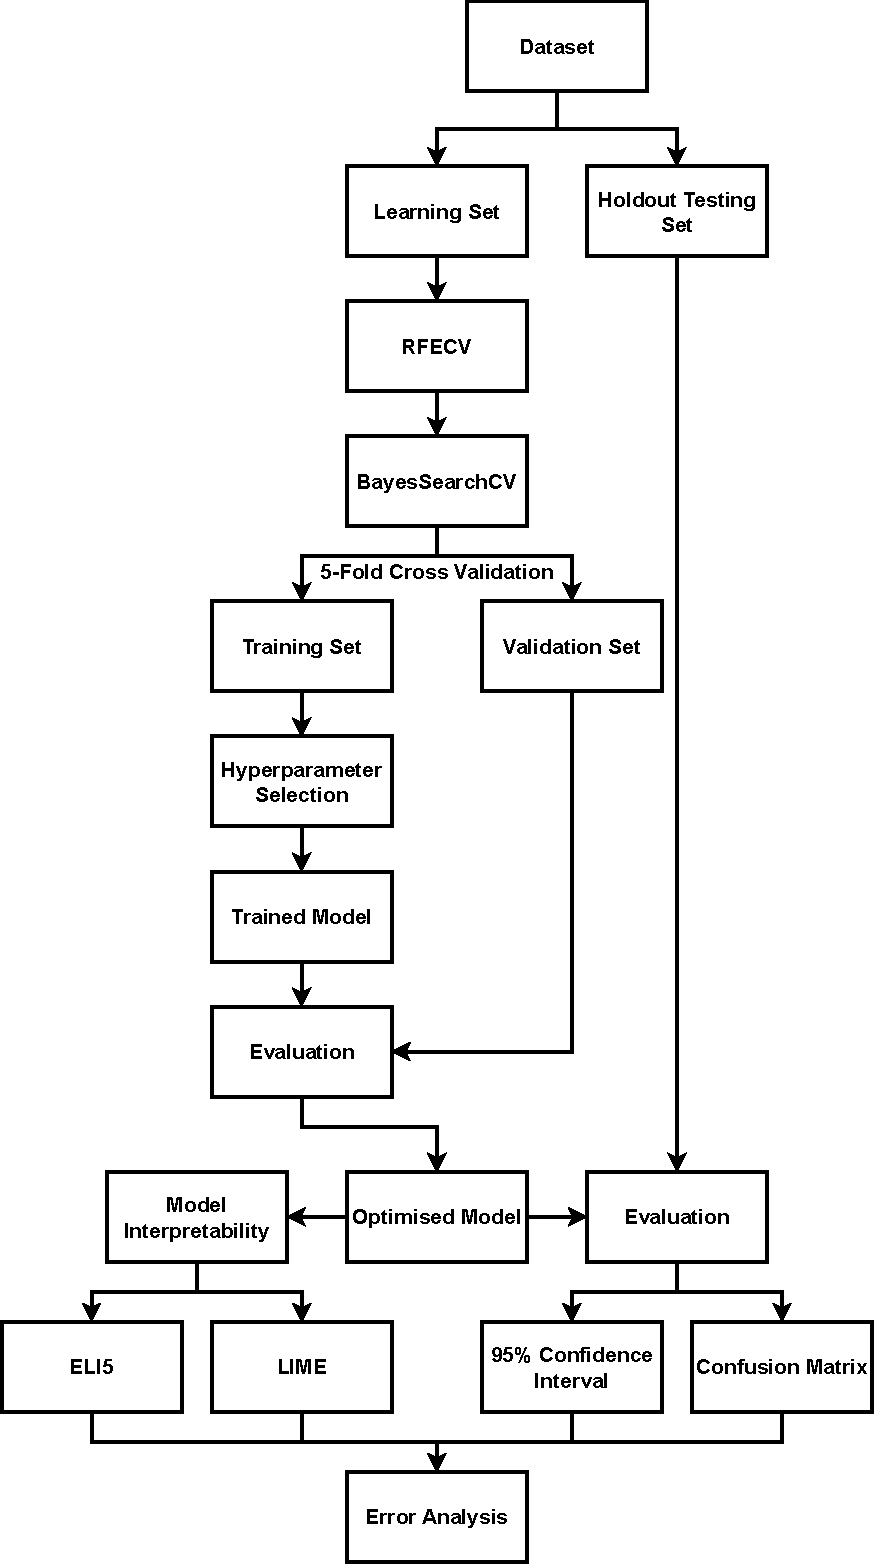
\includegraphics[width=0.85\linewidth]{images/Model_Training.pdf}    
    \caption{Figure showcasing our model training process.}
    \label{fig:Model_Training} 
\end{figure}



% \begin{table}[!h]
% \centering
% \begin{tabular}{lr}
% \toprule
%               Descriptor &  Dimension \\
% \midrule
%          MolecularWeight &       1 \\
%                    XLogP &       1 \\
%                ExactMass &       1 \\
%         MonoisotopicMass &       1 \\
%                     TPSA &       1 \\
%               Complexity &       1 \\
%                   Charge &       1 \\
%          HBondDonorCount &       1 \\
%       HBondAcceptorCount &       1 \\
%       RotatableBondCount &       1 \\
%           HeavyAtomCount &       1 \\
%         IsotopeAtomCount &       1 \\
%          AtomStereoCount &       1 \\
%   DefinedAtomStereoCount &       1 \\
% UndefinedAtomStereoCount &       1 \\
%          BondStereoCount &       1 \\
%   DefinedBondStereoCount &       1 \\
% UndefinedBondStereoCount &       1 \\
%        CovalentUnitCount &       1 \\
%                 Volume3D &       1 \\
%      XStericQuadrupole3D &       1 \\
%      YStericQuadrupole3D &       1 \\
%      ZStericQuadrupole3D &       1 \\
%           FeatureCount3D &       1 \\
%   FeatureAcceptorCount3D &       1 \\
%      FeatureDonorCount3D &       1 \\
%      FeatureAnionCount3D &       1 \\
%     FeatureCationCount3D &       1 \\
%       FeatureRingCount3D &       1 \\
% FeatureHydrophobeCount3D &       1 \\
%     ConformerModelRMSD3D &       1 \\
%    EffectiveRotorCount3D &       1 \\
%         ConformerCount3D &       1 \\
%            Fingerprint2D &     881 \\
% \bottomrule
% \end{tabular}
% \caption{Drug descriptors extracted from PubChem \citep{PubChem}.}
% \label{tbl:PubChem_Descriptors}
% \end{table}

% \begin{table}[!h]
% \centering
% \begin{tabular}{lr}
% \toprule
% Amino Acid Descriptors &  Dimension \\
% \midrule
%     crucianiProperties &       3 \\
%          kideraFactors &      10 \\
%                zScales &       5 \\
%                 FASGAI &       6 \\
%                tScales &       5 \\
%                   VHSE &       8 \\
%                 protFP &       8 \\
%               stScales &       8 \\
%                 BLOSUM &      10 \\
%                 MSWHIM &       3 \\
%                 PSSM   &       - \\
% \bottomrule
% \end{tabular}
% \caption{Amino acid descriptors calculated using the \citet{Peptides} and Protr \citep{ProtR_Paper} R libraries.}
% \label{tbl:Amino_Acid_Descriptors}
% \end{table}

% \begin{table*}
% \centering
% \begin{tabular}{llr}
% \toprule
% Protein Sequence Descriptor Family &      Protein Sequence Descriptor &  Dimension \\
% \midrule
%             Amino acid composition &           Amino acid composition &      20 \\
%                                    &            Dipeptide composition &     400 \\
%                                    &           Tripeptide composition &    8000 \\
%                                    &          Normalized Moreau-Broto &     240 \\
%                    Autocorrelation &                            Moran &     240 \\
%                                    &                            Geary &     240 \\
%                                    &                      Composition &      21 \\
%                                CTD &                       Transition &      21 \\
%                                    &                     Distribution &     105 \\
%                     Conjoint Triad &                   Conjoint Triad &     343 \\
%               Quasi-sequence-order &   Sequence-order-coupling number &      60 \\
%                                    & Quasi-sequence-order descriptors &     100 \\
%      Pseudo-amino acid composition &                           Type I &      50 \\
%                                    &                          Type II &      80 \\
% \bottomrule
% \end{tabular}
% \caption{Protein sequence descriptors calculated using the Protr \citep{ProtR_Paper} R library.}
% \label{tbl:ProtR_Descriptors}
% \end{table*}

\subsection{Streamlit Web App Development}

As mentioned in Subsection \ref{subsubsec:Presenting_Findings} the web app was created to summarise our work and to allow users to perform predictions using our trained models, excluding the neural networks which could not be provided due to size constraints.

We should mention that the model interpretability tools we have already discussed in Subsection \ref{subsubsec:Interpretability} were also made available but not every model can make use of them. \href{https://alphafold-dataset-drug-binding-prediction.streamlit.app/}{\textbf{You can access our web app using this link}}